% Chapter Template

\chapter{Implementation} % Main chapter title

\label{sec:Implementation} % Change X to a consecutive number; for referencing this chapter elsewhere, use \ref{ChapterX}

%----------------------------------------------------------------------------------------
%	SECTION 1
%----------------------------------------------------------------------------------------

%\section{Code organisation}

The code I have developed for this project is all publicly available on my github page (\cite{FB}). It can easily be installed using the setup file provided, which makes it easy to then use Python's customary import command to play with the code.
The code is organised in several sub modules and makes use of factories in plenty of places so that I can easily try out different puzzles, dimensions, search techniques, heuristics, network architecture, etc... without having to change anything except the parameters passed in the command line. Here is a visual overview of the code base with the main dependencies between the main submodules and classes. Solid arrows indicate inheritance (e.g. AStar inherits from SearchStrategy), while dotted lines indicate usage (e.g. AStar uses Heuristic, DeepReinforcementLearner uses DeepLearning, etc..).



\begin{figure}[H]
  \noindent
  \makebox[\textwidth]{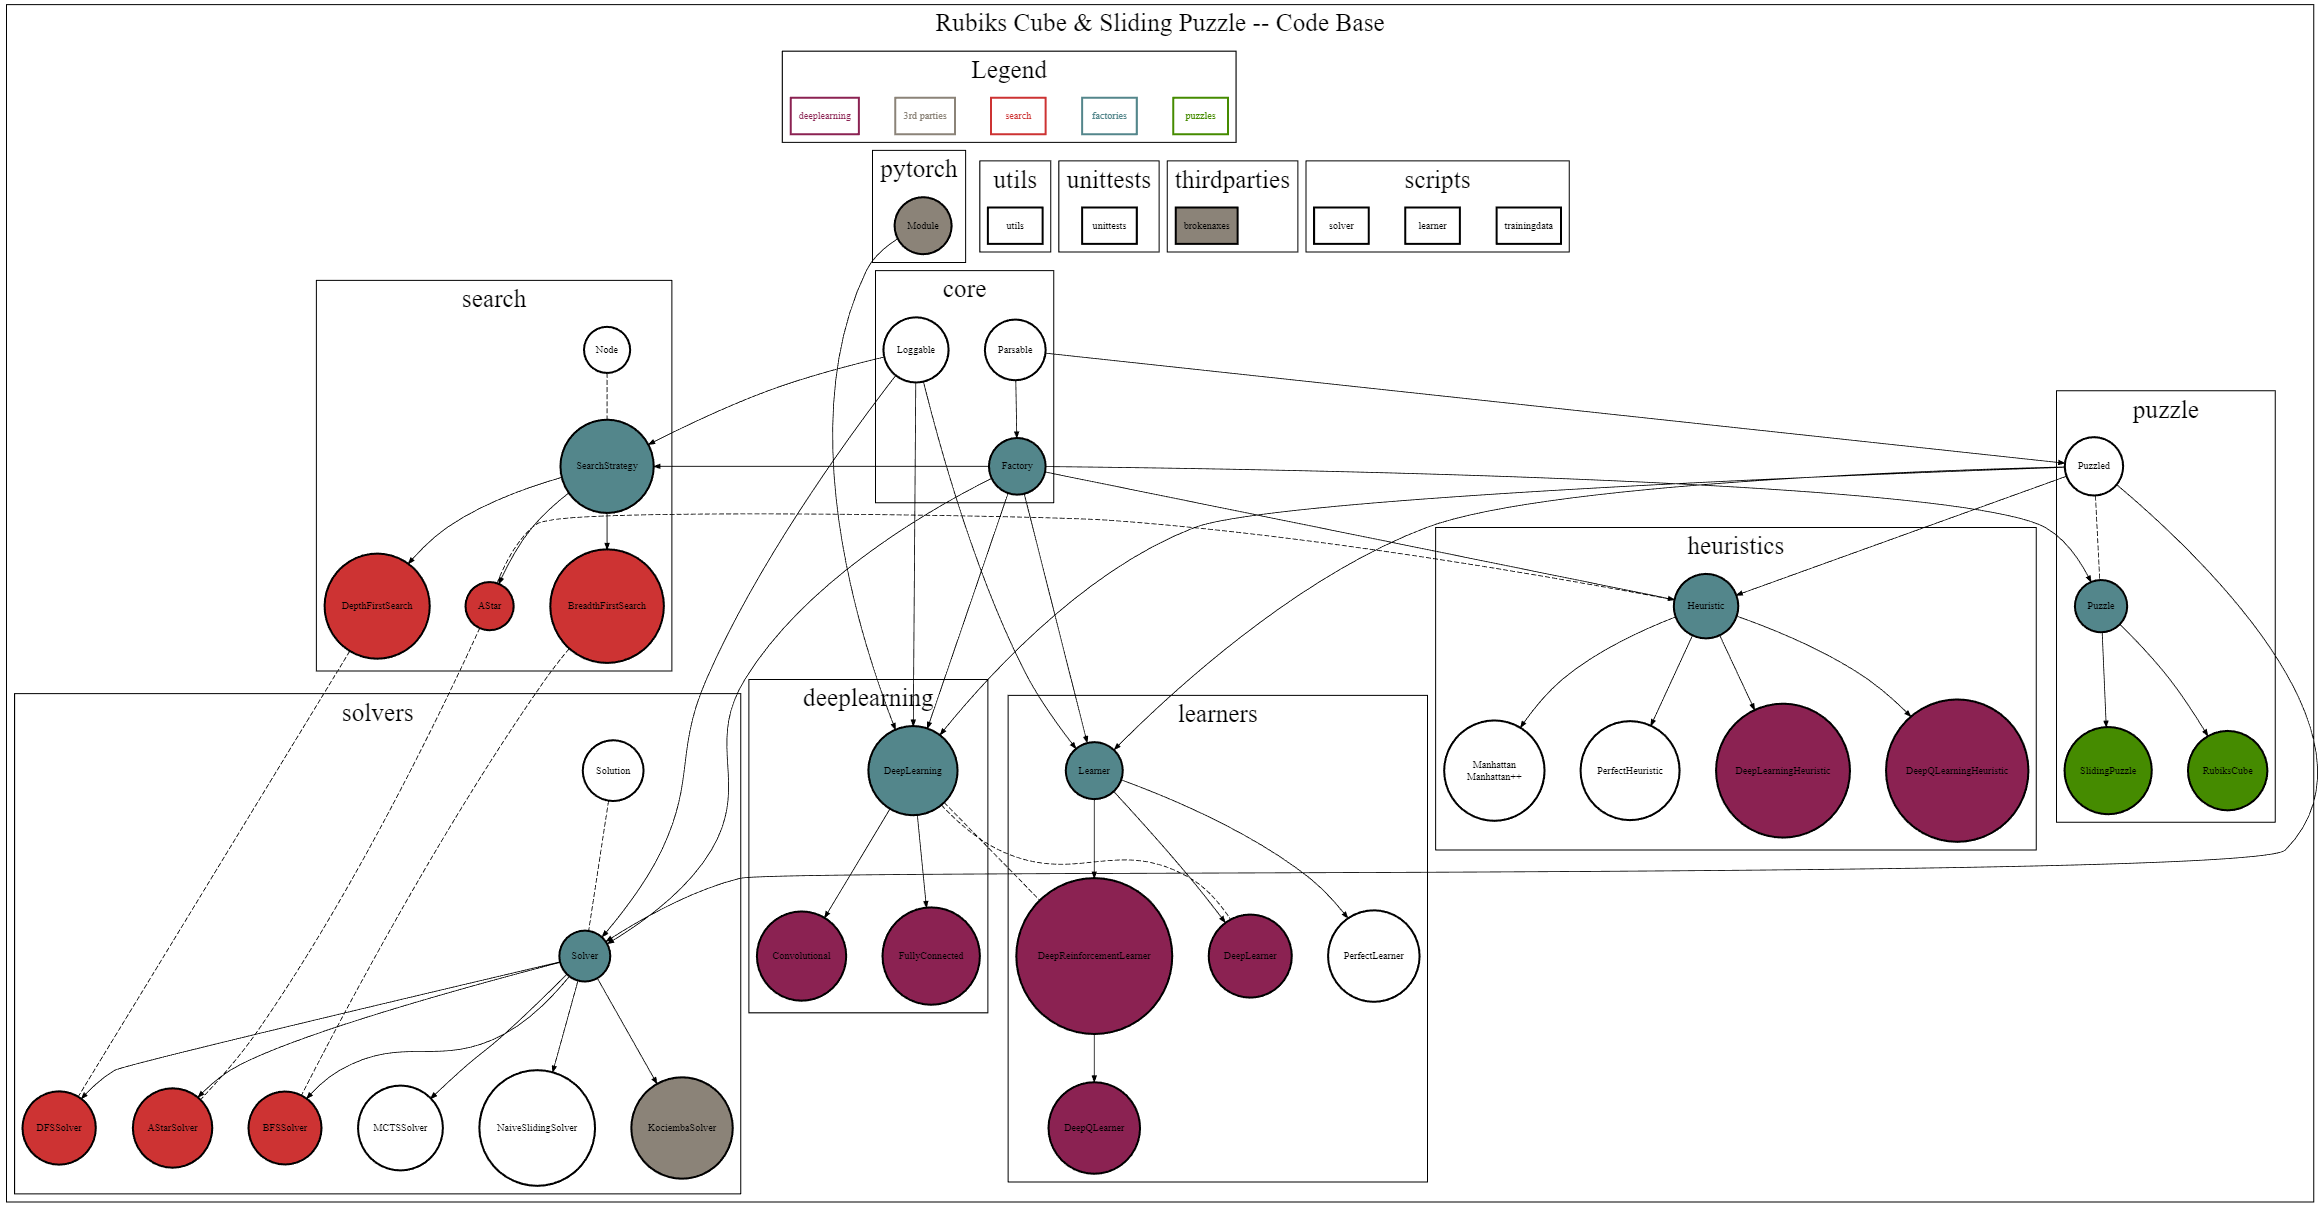
\includegraphics[scale=0.5]{./Figures/codebase}}
  \caption[Codebase]{Code base}
  \label{fig:Codebase}
\end{figure}


\noindent Let me now describe what each submodule does in more details:

\Section{rubiks.core}
\begin{figure}[H]
\centering
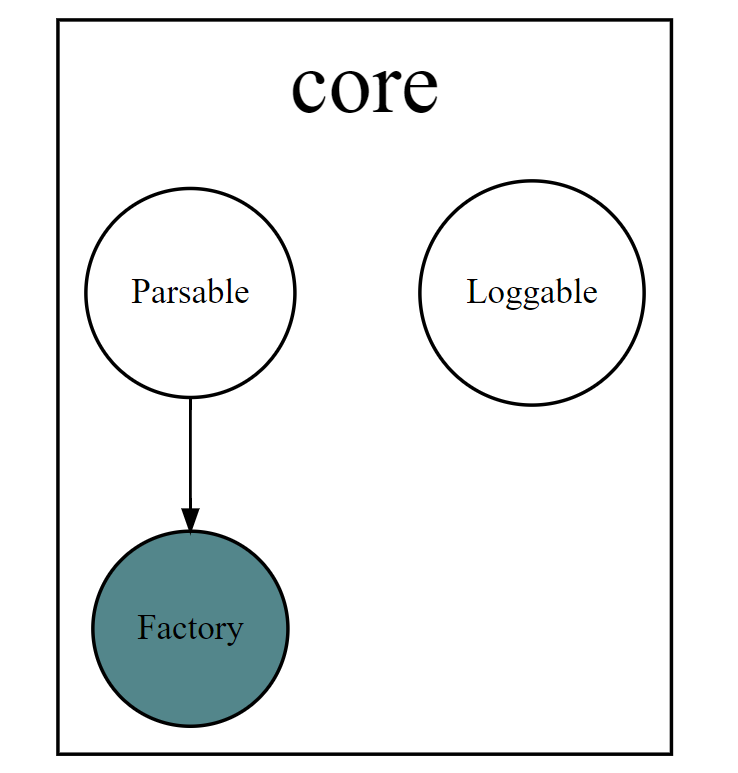
\includegraphics[scale=0.22]{./Figures/codebasecore}
%\decoRule
\caption[Codebase]{rubiks.core}
\label{fig:Codebasecore}
\end{figure}
This submodule contains base classes that make the code base easier to use, debug, and extend. It contains the following:
\begin{itemize}
\item \textbf{Loggable}: a wrapper around Python's logger to automatically picks up classes' names at init and format things nicely (dict, series and dataframes in particular).
\item \textbf{Parsable}: a wrapper around ArgumentParser, which allows to construct objects in the project from command line, to define dependencies between object's configurations and to help a bit with typing of configs. The end result is that you can pretty much pass **kw\_args everywhere and it just works.
\item \textbf{Factory}: a typical factory pattern. Concrete factories can just define what widget they produce and the factory will help construct them from **kw\_args (or command line, since Factory inherits from Parsable)
\end{itemize}


\Section{rubiks.puzzle}
\begin{figure}[H]
\centering
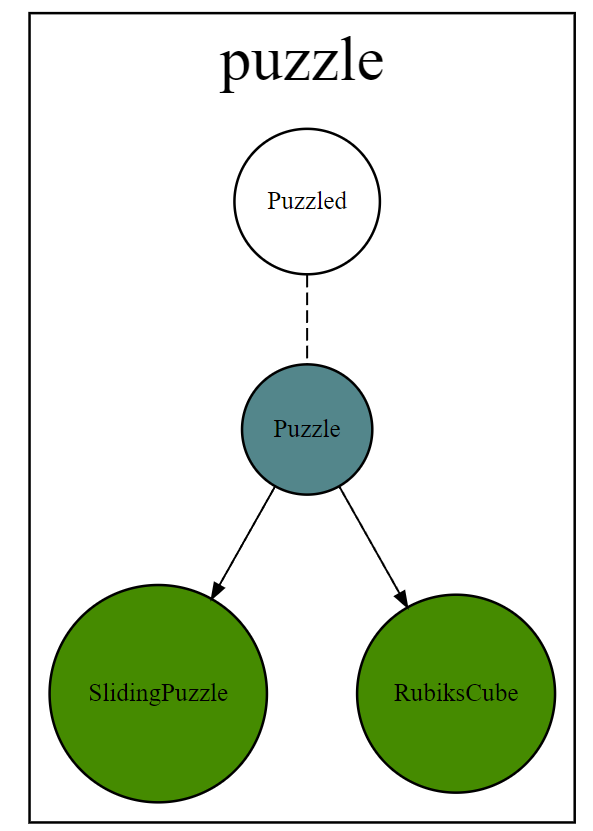
\includegraphics[scale=0.22]{./Figures/codebasepuzzle}
%\decoRule
\caption[Codebase]{rubiks.puzzle}
\label{fig:Codebasepuzzle}
\end{figure}
This submodule contains:
\begin{itemize}
\item \textbf{Puzzle}: a Factory of puzzles. It defines states and actions in the abstract, and provides useful functions to apply moves, shuffle, generate training sets, tell if a state is the goal, etc. Puzzle can manufacture the two following types of puzzles:
\item \textbf{SlidingPuzzle}. Implements the states and moves of the sliding puzzle.
\item \textbf{RubiksCube}. Implements the states and moves of the Rubik's cube.
\\
\\
In addition, this module contains a \textbf{Puzzled} base class which most classes below inherit from. That allow e.g. heuristics, search algorithms, solvers and learners to know what puzzle and dimension they operate on, without having to reimplement these basic facts in each of them.
\end{itemize}

\Section{rubiks.search}
\begin{figure}[H]
\centering
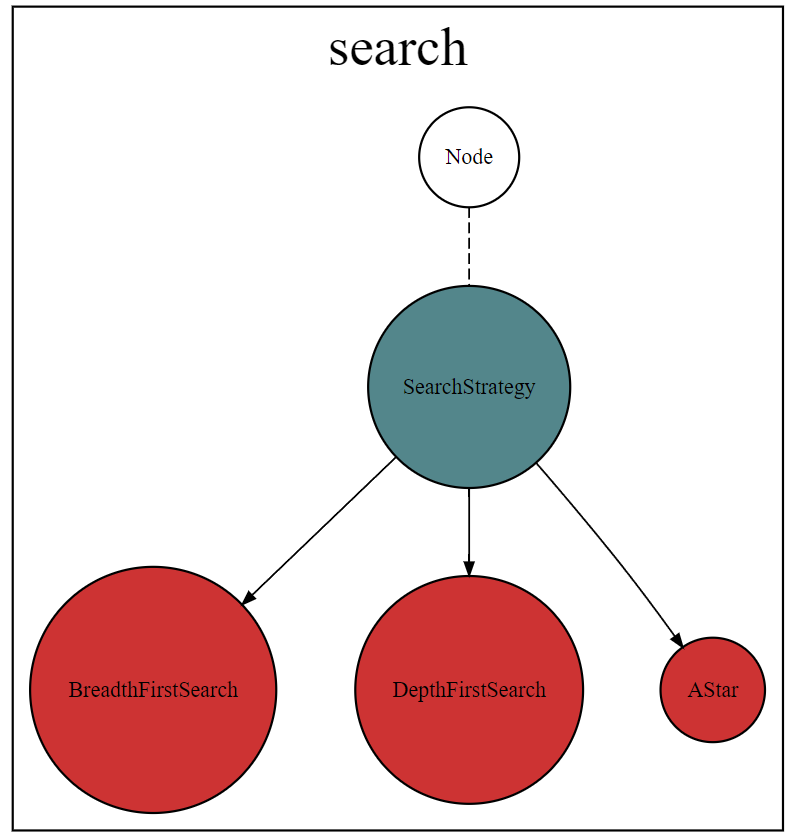
\includegraphics[scale=0.22]{./Figures/codebasesearch}
%\decoRule
\caption[Codebase]{rubiks.search}
\label{fig:Codebasesearch}
\end{figure}
This modules contains graph search strategies. I have actually reused the code I implemented for one of the AIPnT assignments here. It contains the following classes:
\begin{itemize}
\item \textbf{Node}: which contains the state of a graph, as well as link to the previous (parent) state, action that leads from the latter to the former and the cost of the path so far.
\item \textbf{SearchStrategy}, a Factory class which can instantiate the following three types of search strategies to find a path to a goal:
\item \textbf{BreadthFirstSearch}, which is obviously an optimal strategy, but not particularly efficient.
\item \textbf{DepthFirstSearch}, which is not an optimal strategy, and also generally not particularly efficient.
\item \textbf{AStar}, which is optimal, and as efficient as the heuristic it makes use of is.
\end{itemize}

\Section{rubiks.heuristics}
\begin{figure}[H]
\centering
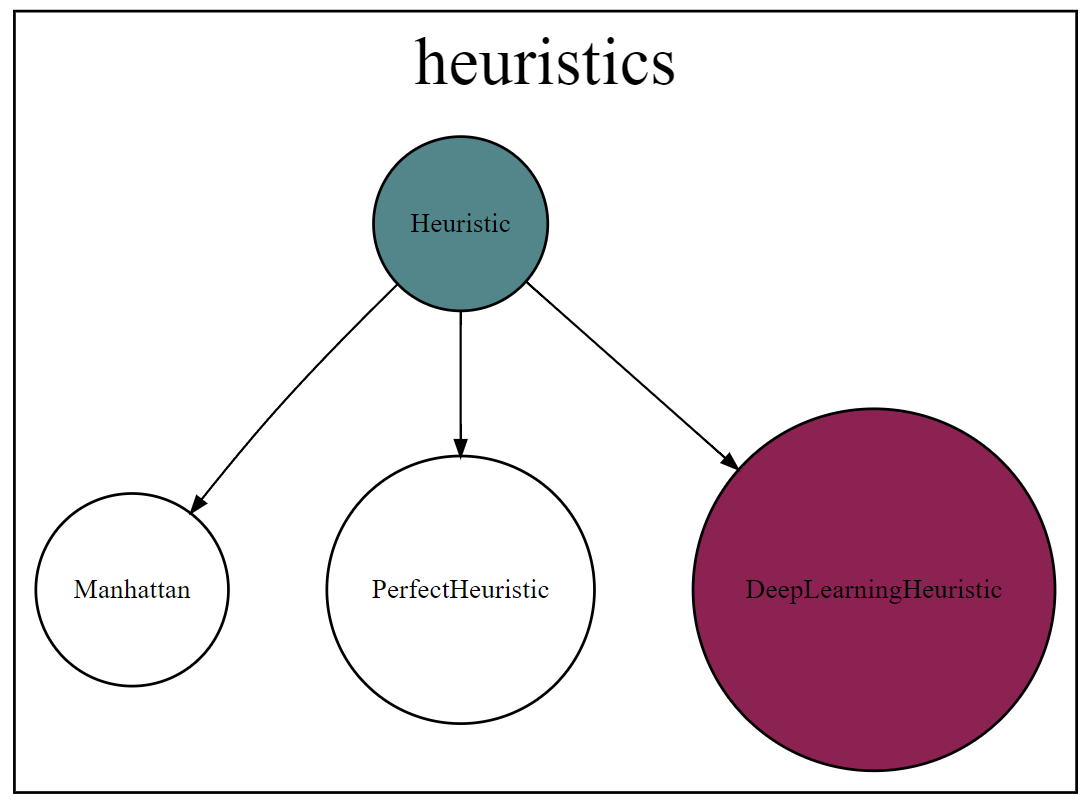
\includegraphics[scale=0.22]{./Figures/codebaseheuristics}
%\decoRule
\caption[Codebase]{rubiks.heuristics}
\label{fig:Codebaseheuristics}
\end{figure}
\label{HSS}
This module contains base class Heuristic, also a Factory. Heuristic can instantiate the following heuristics, which we can use in the AStar strategy from the previous section:
\begin{itemize}
\item \textbf{Manhattan}: This heuristic is specific to the SP. It simply adds for each tile (other than the empty tile) the $L_{1}$ distance between their current position and their target position. We can quickly see that this heuristic is admissible. Indeeed, each move displaces one (and one only) tile by one position. In other puzzles, it is generally the case that a move will affect the position of many tiles (e.g. RC). Therefore, if tiles could somehow freely move on top of one-another (that is, we remove the constraint that there can be at most one tile per compartment, the number of moves necessary to solve the \textbf{SP} would exactly be the Manhattan distance.
\\
\\
The reason why it is interesting to have a known admissible heuristic is that we can obvioulsy compare other heuristics (DL, DRL, DQL, etc) in terms of optimality.
\\
\\
I have also implemented an improvement to the Manhattan distance, which I shall call Manhattan++ in here (and in code logs and graphs) and can be activated by simply passing \textit{plus=True} to the Manhattan Heuristic (see example \ref{ASSS} as well as a thorougher performance comparison on the 2x5 \textbf{SP} in \ref{MHComp}). It is based on the concept of linear constraints that I read about in lecture notes from Washington University (\cite{SlidingPuzzleLectureNotes}). The idea is simply that when tiles are already placed on their target row or column, but not in the expected order, we will need to get the tiles out of the way of one another to get to the goal state, and this is not accounted for by the Manhattan distance. For instance, in the following 2x3 puzzle, the Manhattan distance does not account for the fact that, at best, tile \red 3 \black needs to get out of the way for tiles \blue 1 \black and \blue 2 \black to move, and then needs to get back in its row, adding a cost of 2 to the Manhattan distance.

\begin{center}
\begin{five}
\setrow{2}{\red 3, \blue 1, \blue 2}
\setrow{1}{4, 5, 0}
\end{five}
\end{center}

Two important things to notice are that linear constraints across rows and columns (which I might generically refer to as \textit{lines} in the following) can be added without breaking admissibility (hence giving more pessimistic, or accurate, cost estimates than simple Manhattan). This is because if a tile is involved in two linear constraints, it will need to get out of the way both horizontally and vertically. The second thing is that when several pairs in a line are not in order, we cannot simply add 2 for each distinct out-of-order pair, the right penalty to add is more subtle than that and needs to be computed recursively. For instance, let us now consider the following configuration:
\begin{center}
\begin{five}
\setrow{2}{\red 3, \red 2, \red 1}
\setrow{1}{4, 5, 0}
\end{five}
\end{center}
The correct penalty to add is not 6 (3 times 2 since all pairs (1, 2), (1, 3) and (2, 3) are out of order, but only 4. Indeed if, say, tile 3 got somehow out of the way at the back of the SP (imagine just another dimension there where we can move tiles) and tile 2 got out of the way by moving down to let tile 1 pass across, we could be done by simply adding 4 to the Manhattan distance (2 to move tile 3 out and back, and 2 to move tile 2 out and back). The correct way to compute the penalty cost for linear constraints is therefore to do it recursively, taking the minimum additional cost of moving either the left-most or the right-most tile of the line under consideration out of the way (that additional cost to move these left-most or right-most tile is 2 if not at their expected order in the line, 0 otherwise) plus the penalty of reordering the rest of the line.
\\
\\
Finally, as suggested by the reference lecture notes (which give very vague details about the above subtleties), I have precomputed all the penalties for all possible rows, columns and all possible tiles ordering they could have and saved the corresponding penalties in a database. For memory efficiency, I also only saved penalties which are non-zero. The very first time any call to Manhattan++ is made, for a given dimension nxm, the appropriate linear constraint penalties are computed and populated in a database.
\\
\\
Notice that for an nxm \textbf{SP}, there are n rows, each of which can have $\frac{(n * m)!}{(n * m - m)!}$ different ordering of tiles and m columns which can each have $\frac{(n * m)!}{(n * m - n)!}$ different ordering of tiles. This means the pre-computations and data-base sizes for the Manhattan++ heuristic are actually manageable, as it grows much slower than the number of possible puzzles. The maximum number of penalties to compute for $nxm \leq 5x5$ are:


\begin{center}
\begin{tabular}{l*{6}{c}r}
n              & m & 2 & 3 & 4 & 5\\
\hline
2              &   & 48 & 330 & 3,584 & 60,930 \\
3              &   &   & 3,024  & 40,920 &  1,094,730  \\
4              &   &   &  & 349,440 & 8,023,320   \\
5              &   &   &  &  & 63,756,000   \\
\end{tabular}
\end{center}
Taking also into account that we only store non-zero penalties, we actually get the following (quite smaller) number of penalties in our data bases:
\begin{center}
\begin{tabular}{l*{6}{c}r}
n              & m & 2 & 3 & 4 & 5\\
\hline
2              &   & 2 & 46 & 1,238  & 32,888 \\
3              &   &  & 278  & 7,122 & 328,894   \\
4              &   &   &  & 40,546 &  1,456,680 \\
5              &   &   &  &  &  8,215,382 \\
\end{tabular}
\end{center}



\item \textbf{PerfectHeuristic}: this reads from a data base the optimal costs, pre-computed by the PerfectLearner (see below \ref{PLcode})
\item \textbf{DeepLearningHeuristic}: this uses a network which has been trained using \textbf{DL} (DeepLearner) \textbf{DRL} (DeepReinforcementLearner) or \textbf{DQL} (DeepQLearner). See \ref{DRLcode} for a discussion of these three learners.
\item \textbf{DeepQLearningHeuristic}: this uses a network which has been trained using \textbf{DQL} by the DeepQLearner (see below \ref{DQLcode}). The DeepQLearningHeuristic follows the same interface as the other heuristics, and therefore can be used by A$^{*}$ for instance. It also has an additional method \textit{optimal\_actions} that returns the learnt probability distribution over actions for a given puzzle, for use in search algorithms (e.g. \textbf{MCTS}) which make use of this to inform their search.
\end{itemize}



\Section{rubiks.deeplearning}
\begin{figure}[H]
\centering
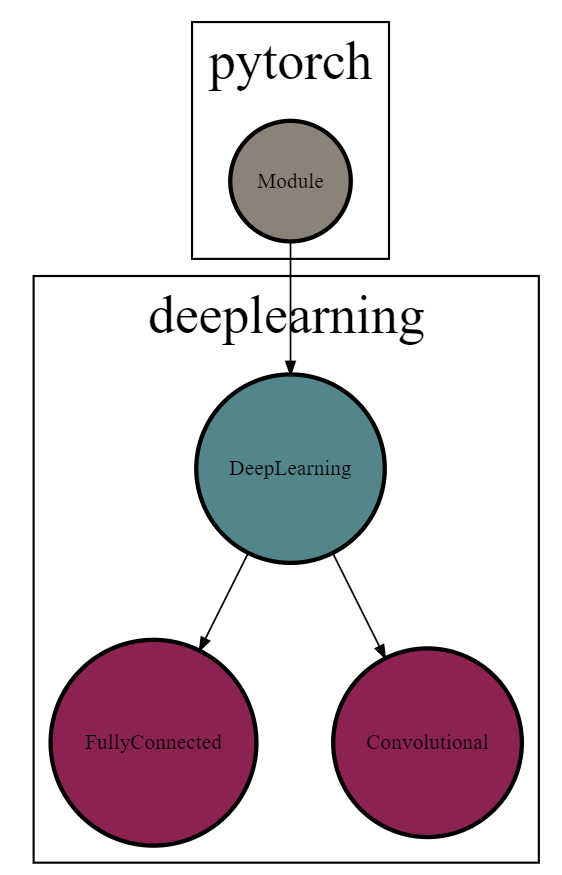
\includegraphics[scale=0.22]{./Figures/codebasedeeplearning}
%\decoRule
\caption[Codebase]{rubiks.deeplearning}
\label{fig:Codebasedeeplearning}
\end{figure}
This module is a wrapper around Pytorch. It contains:
\begin{itemize}
\item \textbf{DeepLearning}: a Puzzled Loggable Factory that can instantiate some configurable deep networks, and provide the necessary glue with the rest of the code base so that puzzles be seemlessly passed to the networks and trained on. 
\item \textbf{FullyConnected}: wrapper around a Pytorch fully connected network, with configurable hidden layers and size. Parameters allow to add drop out, to indicate whether or not the inputs are one hot encoding (in which case the first layer is automatically adjusted in size, using information from the puzzle dimension). There is also importantly a \textit{joint\_policy} parameter to indicate whether we want the output to be 1 dimensional (e.g. for value function learning) or $a+1$-dimensional, where $a$ is the size of the actions space (for joint policy-value learning).
\item \textbf{Convolutional}: similar wrapper to FullyConnected, but with the ability to add some parallel convolutional layers to complement fully connected layers.
\end{itemize}


\Section{rubiks.learners}
\label{sec:codelearners}
\begin{figure}[H]
\centering
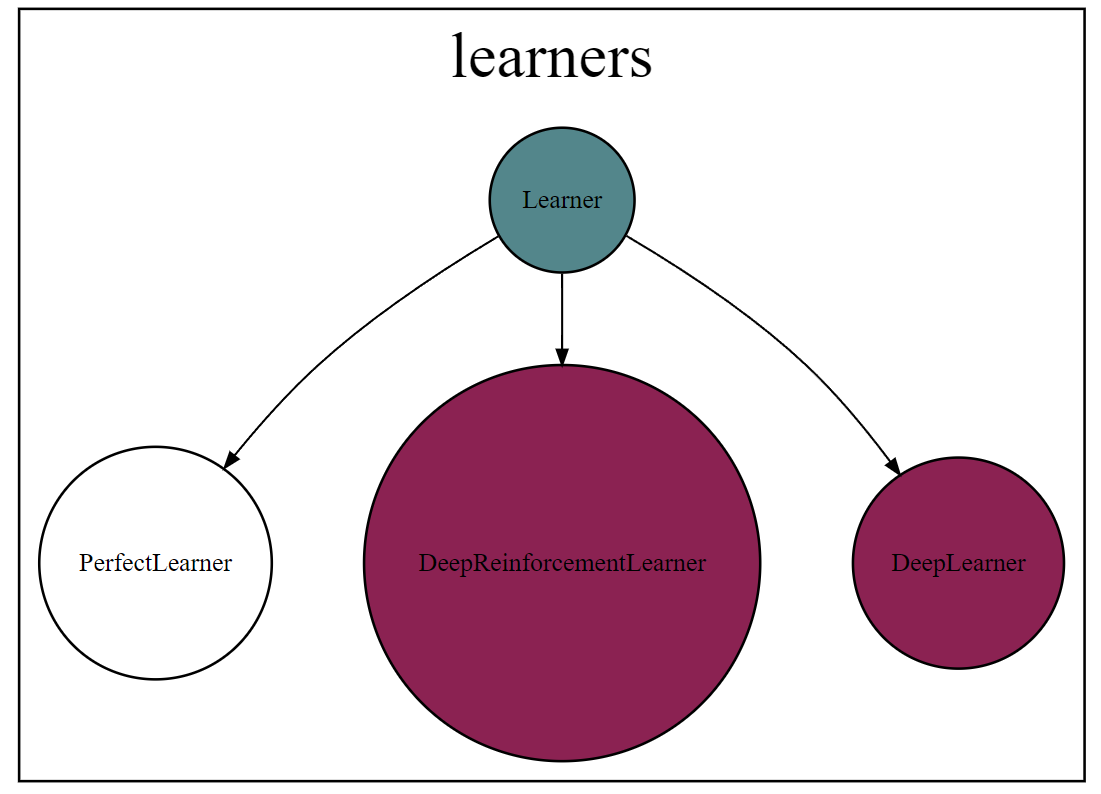
\includegraphics[scale=0.22]{./Figures/codebaselearners}
%\decoRule
\caption[Codebase]{rubiks.learners}
\label{fig:Codebaselearners}
\end{figure}
\label{PLcode}
\label{DRLcode}
\label{DQLcode}
This module implements learners, which learn something from a puzzle, store what they learnt, and can display interesting things about what they learnt.

\begin{itemize}
\item \textbf{Learner} is a Puzzled Loggable Factory. It provides some common code to learners (to save or purge what they learnt), kick off learning and plot results. Concrete derived implementation define what and how they learn, and what interesting they can display about this learning process. The four implemented learners are:
\item \textbf{PerfectLearner}: It instantiates an optimal solver ($A^{*}$ with a configurable heuristic - but will only accept heuristic that advertise themselves as optimal. The learning consists in generating all the possible configuration of the considered puzzle, solve them with the optimal solver, and save the optimal cost of it as well as those of the whole solution path. The code allows for parallelization, stop and restart so that we can run on several different occasions and keep completing a database of solutions if necessary or desired. Once the PerfectLearner has completed its job, it can display some interesting information, such as the puzzle's God's number, the distribution of number of puzzles versus optimal cost, the hardest configuration it came across, and how long it took it to come up with the full knowledge of that puzzle. I will show in section \ref{PLSS} how to run an example. Notice that for puzzles of too high dimension, where my computing resources will not allow to solve exhaustively all the configurations of a given dimension, this class can still be used to populate a data base of optimal costs, which can then be used by DeepLearner. If it is to be used this way, the PerfectLearner can be configured to use perfectly random configurations to learn from, rather than going through the configurations one by one in a well defined order.

\item \textbf{DeepLearner} DeepLearner instanciates a DeepLarning (neural network), and trains it on training data by minimizing the mean square error between the cost-to-go from the target solver versus the neural network. The main parameters driving this learner are:
\begin{itemize}
\item \textit{training\_data\_from\_data\_base} which controls whether the training samples are generated on the fly via another solver (defaults to A$^{*}[Manhattan++]$ for \textbf{SP} and A$^{*}[Kociemba]$ for \textbf{RC}) or read from a data base (similarly constructed from other solvers, but has the advantage of being done offline)
\item \textit{nb\_epochs} and \textit{threshold} which control exit criteria for the network training.
\item \textit{nb\_sequences}, \textit{nb\_shuffles\_min}, \textit{nb\_shuffles\_max}, \textit{training\_data\_freq} and \textit{training\_data\_every\_epoch} which control how often we regenerate new training data, how many sequences of puzzles it contais, how scrambled the puzzles should be.
\item \textit{learning\_rate}, \textit{scheduler}, \textit{optimizer} and assorted parameters which control the optimisation at each backward propagation. 
\end{itemize}
Once it has completed (or on a regular basis), DeepLearner saves the trained network, which can then be used with DeepLearningHeuristic to guide A$^{*}$.
\item \textbf{DeepReinforcementLearner}: It instantiates a DeepLearning (network), and trains it using \textbf{DRL} essentially following the pseudo-code from \ref{sec:TheoryDLDRL}. Unlike DeepLearner, the targets are here generated via value iteration rather than via another solver (teacher). It has very similar parameters to the DeepLearner, in particular some parameters to control exit criteria (same as DeepLearner's plus a few that help it exit early when the value function's range has not been increasing anymore for a while), some parameters to control and configure the optimiser, some to control the training puzzles (how many, how often, how scrambled).



\item \textbf{DeepQLearner}: The implementation of the DeepQLearner is actually only a few lines of code, for it inherits pretty much all of its behaviour from the DeepReinforcementLearner. The only overwritten functions are:

\begin{itemize}
\item \textit{get\_loss\_function} which constructs the loss function to be used by the network's training. Instead of returning a simple torch.nn.MSELoss, it returns a function which computes the average of torch.nn.MSELoss on the value-function and torch.nn.CrossEntropyLoss on the actions.
\item \textit{\_\_construct\_target\_\_} which performs the the Q-V-iteration to update the targets, as described in pseudo code form in \ref{sec:TheoryDQL}. This function updates not only the value function of a node given its children nodes, but also updates the optimal action vector (0 for non optimal actions, 1 for the optimal action leading to the child node of highest value function).
\end{itemize} 


\end{itemize}


\Section{rubiks.solvers}
\label{sec:codesolvers}
\begin{figure}[H]
\centering
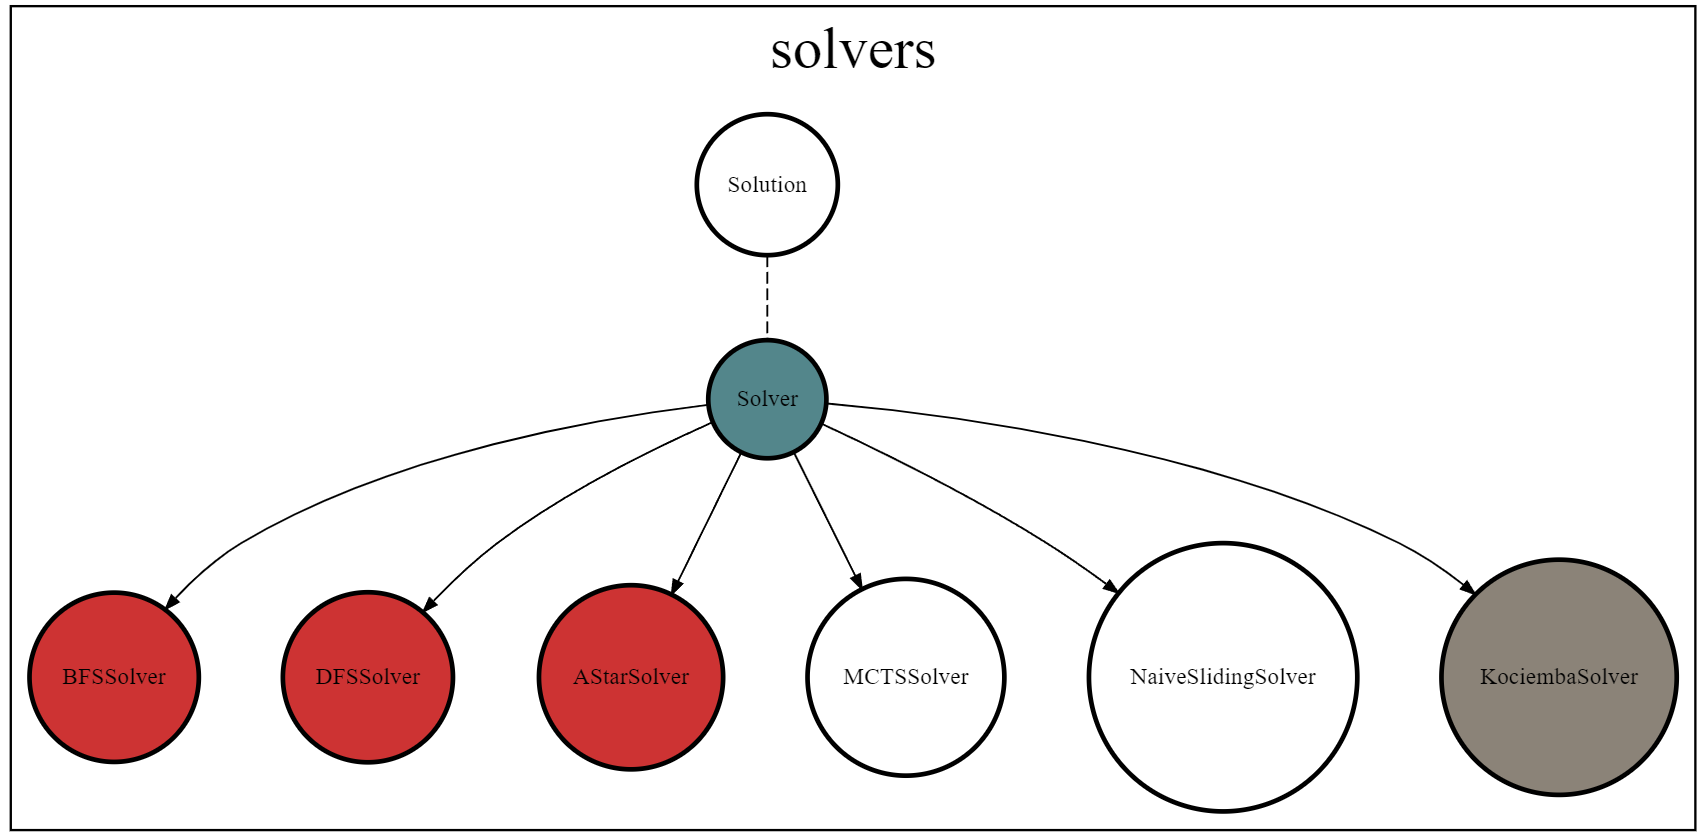
\includegraphics[scale=0.22]{./Figures/codebasesolvers}
%\decoRule
\caption[Codebase]{rubiks.solvers}
\label{fig:Codebasesolvers}
\end{figure}
This module implements the actual puzzles solvers. The base class Solver is a Factory, and in addition to being able to instantiating the following types of solvers, can run different solvers through a similal sequences of random puzzles (for various increasing degrees of difficulty (scrambling), and/or perfectly shuffled ones) and display a comparison of how they perform in a number of metrics (configurable from percentage of puzzles solved before time out, percentage of optimal puzzle (if optimality can be ascertained), mean-median-maximum run time, mean-median-maximum expanded nodes (for solvers where it makes sense), mean-median-max cost, and an optimality score which compares the total sum of cost over all puzzles versus a benchmark solver). Ideally the benchmark solver to compute the optimality score should provably optimal, but in the case of the \textbf{RC} that was not possible so I used A$^{*}$ with KociembaHeuristic as my benchmark. For the \textbf{SP} I used the optimal A$^{*}$ with Manhattan++ heuristic.

\begin{itemize}
\item \textbf{DFSSolver} This solver is literally a few lines of code, extremely close to the pseudo code detailed in \ref{alg:TheoryBFSDFS}
\item \textbf{BFSSolver} Ditto, see \ref{alg:TheoryBFSDFS}
\item \textbf{AStarSolver} Ditto, see \ref{alg:TheoryAStar}
\item \textbf{NaiveSlidingSolver} The NaiveSolver is conceptually simple, but was far from trivial to implement and debug. Its functioning is detailed in the appendix section \ref{sec:Examples}. Basically, it does what a beginner player would do, certainly what I do when I play the sliding puzzle: solving the top row first, then the left column, hence reducing the puzzle to a smaller dimensional one, and keep iterating until done.
\item \textbf{KociembaSolver} This solver is a wrapper around two libraries. The first one, hkociemba (see \cite{HKociemba}) is a 2x2x2 implementation written by Kociemba himself, the second one is a Python pip-installable library which solves the 3x3x3 Rubik's. My  wrapper simply translates my cube representation in that accepted by these 2 solvers, and their result string into moves usable by my code. I also do some additional massaging for the 3x3x3 case, due to a shortcoming/bug in the 3x3x3 Python library, as I have detailed in appendix \ref{sec:Kociemba}.
\item \textbf{MonteCarloSearchTreeSolver} My implementation follows McAleer \& Agostilenni et al \cite{https://doi.org/10.48550/arxiv.1805.07470} but is however single-threaded. As a consequence, I dropped the $\nu$ parameter from their implementation, since it only introduces a penalty to discourage parallel threads from generating the same paths (in single threaded mode, this parameter is inconsequential).
\\
This solver basically generates \textit{pseudo-random} paths from initial node to a new leaf at each iteration (see \ref{alg:TheoryMCTS}), until we obtain a goal leaf.Paths are, despite the name, completely deterministic: they indeed result from a trade-off between the probability of actions (penalised for repeated use) and the value function, but there are no random draws being performed.
\\ As per McAleer \& Agostilenni's paper, I have implemented a final pruning via \textbf{BFS} of the tree resulting from the above \textit{Monte-Carlo} process.It is inded clear that the paths generated by this \textbf{MCTS} algorithm have little chance of being optimal since there is no correction mechanism to favour shortcuts over long loops. I have however made this \textbf{BFS} trimming optional via a \textit{trim\_tree} parameter to study its effect on solutions' optimality and run time (see results section \ref{sec:MTCSHyperParamsEffect}).
\\
I will study and report on the effect of the trade-off hyper-parameter \textit{c}, and confirm how it affects solutions' quality and run time in section \ref{sec:MTCSHyperParamsEffect}.

\end{itemize}

\Section{data}

The code generates a fair amount of data, in particular:
\begin{itemize}
\item Manhattan++ generates databases of linear constraint penalties (see \ref{HSS})
\item TrainingData: (see e.g. \ref{DLSS}) generates databases of puzzles and their associated costs for later training of a DeepLearner.
\item Learners: DeepLearner, DeepReinforcementLearner, DeepQLearner generate models as well as some convergence data useful to understand how the networks learn. Similarly PerfectLearner saves its results for later reuse (in e.g. PerfectHeuristic) or display.
\item Solver: Generates sequences of scrambled puzzles used to make the performance test (comparing different solvers) fair.
\item Solver.performance\_test: Generates a data frame containing the metrics discussed earlier in \ref{sec:codesolvers}, for each solver and each level of difficulty.
\end{itemize}
That data is saved under a tree following the schema below:
$$\$RUBIKSDATA/data\_type/puzzle\_type/dimension/file\_name.pkl$$

